\chapter{Bugzilla \\
\small{\textit{-- Luo Xu, Gavin Lam, Annanya Jain}
\index{Bugzilla} 
\index{Chapter!Bugzilla}
\label{Chapter::Bugzilla}}}

\section{DigitalOcean Setup}
We made an account in DigitalOcean via GitHub and received 200 credits via student package.

\noindent We created an droplet with these stats: 2 GB Memory / 60 GB Disk / NYC3 - Ubuntu 24.04 (LTS) x64

\section{Bugzilla}
After setting up the droplet, we ssh into the droplet through the local terminal with the public ip: 174.138.68.199. Then I checked the updates, and installed the essential tools and prerequisites.
\begin{minted}{shell}
ssh root@174.138.68.199
apt update
apt upgrade -y
apt install -y git curl wget nano build-essential
apt install -y apache2 libapache2-mod-perl2 \
  mariadb-server mariadb-client \
  libcgi-pm-perl libdbi-perl libdbd-mysql-perl \
  libtemplate-perl libdatetime-perl libdatetime-timezone-perl \
  libemail-sender-perl libemail-mime-perl libxml-twig-perl \
  libgd-perl libjson-xs-perl libauthen-sasl-perl libnet-ldap-perl \
  libsoap-lite-perl libxmlrpc-lite-perl libtest-taint-perl \
  libhtml-scrubber-perl libfile-mimeinfo-perl libcache-memcached-perl \
  perlmagick graphviz lynx python3-sphinx
\end{minted}
I then configured the database.
\begin{minted}{shell}
systemctl start mariadb
systemctl enable mariadb
mysql_secure_installation
\end{minted}
I logged into the database.
\begin{minted}{shell}
mysql -u root -p
\end{minted}
and then inside the shell i set up a user in the SQL shell.
\begin{minted}{sql}
CREATE DATABASE bugzilla;
CREATE USER 'bugzillauser'@'localhost' IDENTIFIED BY '<password here>';
GRANT ALL PRIVILEGES ON bugzilla.* TO 'bugzillauser'@'localhost';
FLUSH PRIVILEGES;
EXIT;
\end{minted}
I downloaded and configured bugzilla.
\begin{minted}{shell}
cd /var/www
git clone https://github.com/bugzilla/bugzilla.git
# Or download a tarball, e.g. wget from bugzilla.org, then extract
\end{minted}
Here was when we realized we might have made an mistake of not running this in docker, so we went to stop the services based on what chat said, and resetted the host services within the droplet.
\begin{minted}{shell}
sudo systemctl stop apache2 || true
sudo systemctl disable apache2 || true
sudo systemctl stop mariadb || true
sudo systemctl disable mariadb || true
\end{minted}
Then we installed docker and all the compose plugins incase we are missing anything. 
\begin{minted}{shell}
sudo apt update
sudo apt install -y ca-certificates curl gnupg
sudo install -m 0755 -d /etc/apt/keyrings
curl -fsSL https://download.docker.com/linux/ubuntu/gpg | \
  sudo gpg --dearmor -o /etc/apt/keyrings/docker.gpg
echo \
  "deb [arch=$(dpkg --print-architecture) signed-by=/etc/apt/keyrings/docker.gpg] \
  https://download.docker.com/linux/ubuntu $(. /etc/os-release; echo $VERSION_CODENAME) stable" | \
  sudo tee /etc/apt/sources.list.d/docker.list > /dev/null
sudo apt update
sudo apt install -y docker-ce docker-ce-cli containerd.io docker-buildx-plugin docker-compose-plugin
\end{minted}
Then I made a project folder and env file.
\begin{minted}{shell}
mkdir -p ~/bugzilla-docker
cd ~/bugzilla-docker

cat > .env << 'EOF'
# ---- DB credentials (choose your own secure values) ----
MYSQL_ROOT_PASSWORD=<password>
BUGZ_DB=bugzilla
BUGZ_USER=bugzillauser
BUGZ_PASS=<password>

# ---- Internal service names / URLs ----
BUGZ_HOST=bugzilla
# If you have a domain now, set https URL. If not, set http://<PUBLIC_IP> for now and change later.
BUGZ_URL=http://<PUBLIC_IP>
EOF
\end{minted}

I created docker-compose.yml.
\begin{minted}{yaml}
services:
  db:
    image: mariadb:10.6
    restart: unless-stopped
    environment:
      MYSQL_ROOT_PASSWORD: ${MYSQL_ROOT_PASSWORD}
      MYSQL_DATABASE: ${BUGZ_DB}
      MYSQL_USER: ${BUGZ_USER}
      MYSQL_PASSWORD: ${BUGZ_PASS}
    command: ["--character-set-server=utf8mb4","--collation-server=utf8mb4_unicode>
    volumes:
      - db_data:/var/lib/mysql
    networks: [bugznet]

  bugzilla:
    image: nasqueron/bugzilla:latest
    depends_on: 
      db:
        condition: service_healthy
    restart: unless-stopped
    environment:
      DB_HOST: db
      DB_USER: ${BUGZ_USER}
      DB_PASSWORD: ${BUGZ_PASS}
      DB_DATABASE: ${BUGZ_DB}
      BUGZILLA_URL: ${BUGZ_URL}
    ports:
      - "80:80"
    volumes:
      - bug_data:/var/www/html/bugzilla
    networks: [bugznet]

volumes:
  db_data:
  bug_data:

networks:
  bugznet:    
\end{minted}

I create the stack and checked the logs for the email and password. 
\begin{minted}{shell}
docker compose down && docker compose up -d
docker compose logs -f bugzilla
docker compose exec -it db bash
docker compose restart bugzilla
docker compose logs -f bugzilla
...
bugzilla-1  | If no admin account is already defined in your database, this one will be created:
bugzilla-1  | 
bugzilla-1  | 	E-mail ..... admin@domain.tld
bugzilla-1  | 	Password ... OdMWObr43g6VW2uG8
...
\end{minted} 


\noindent I then went to the bugzilla site.


\begin{figure}
    \centering
    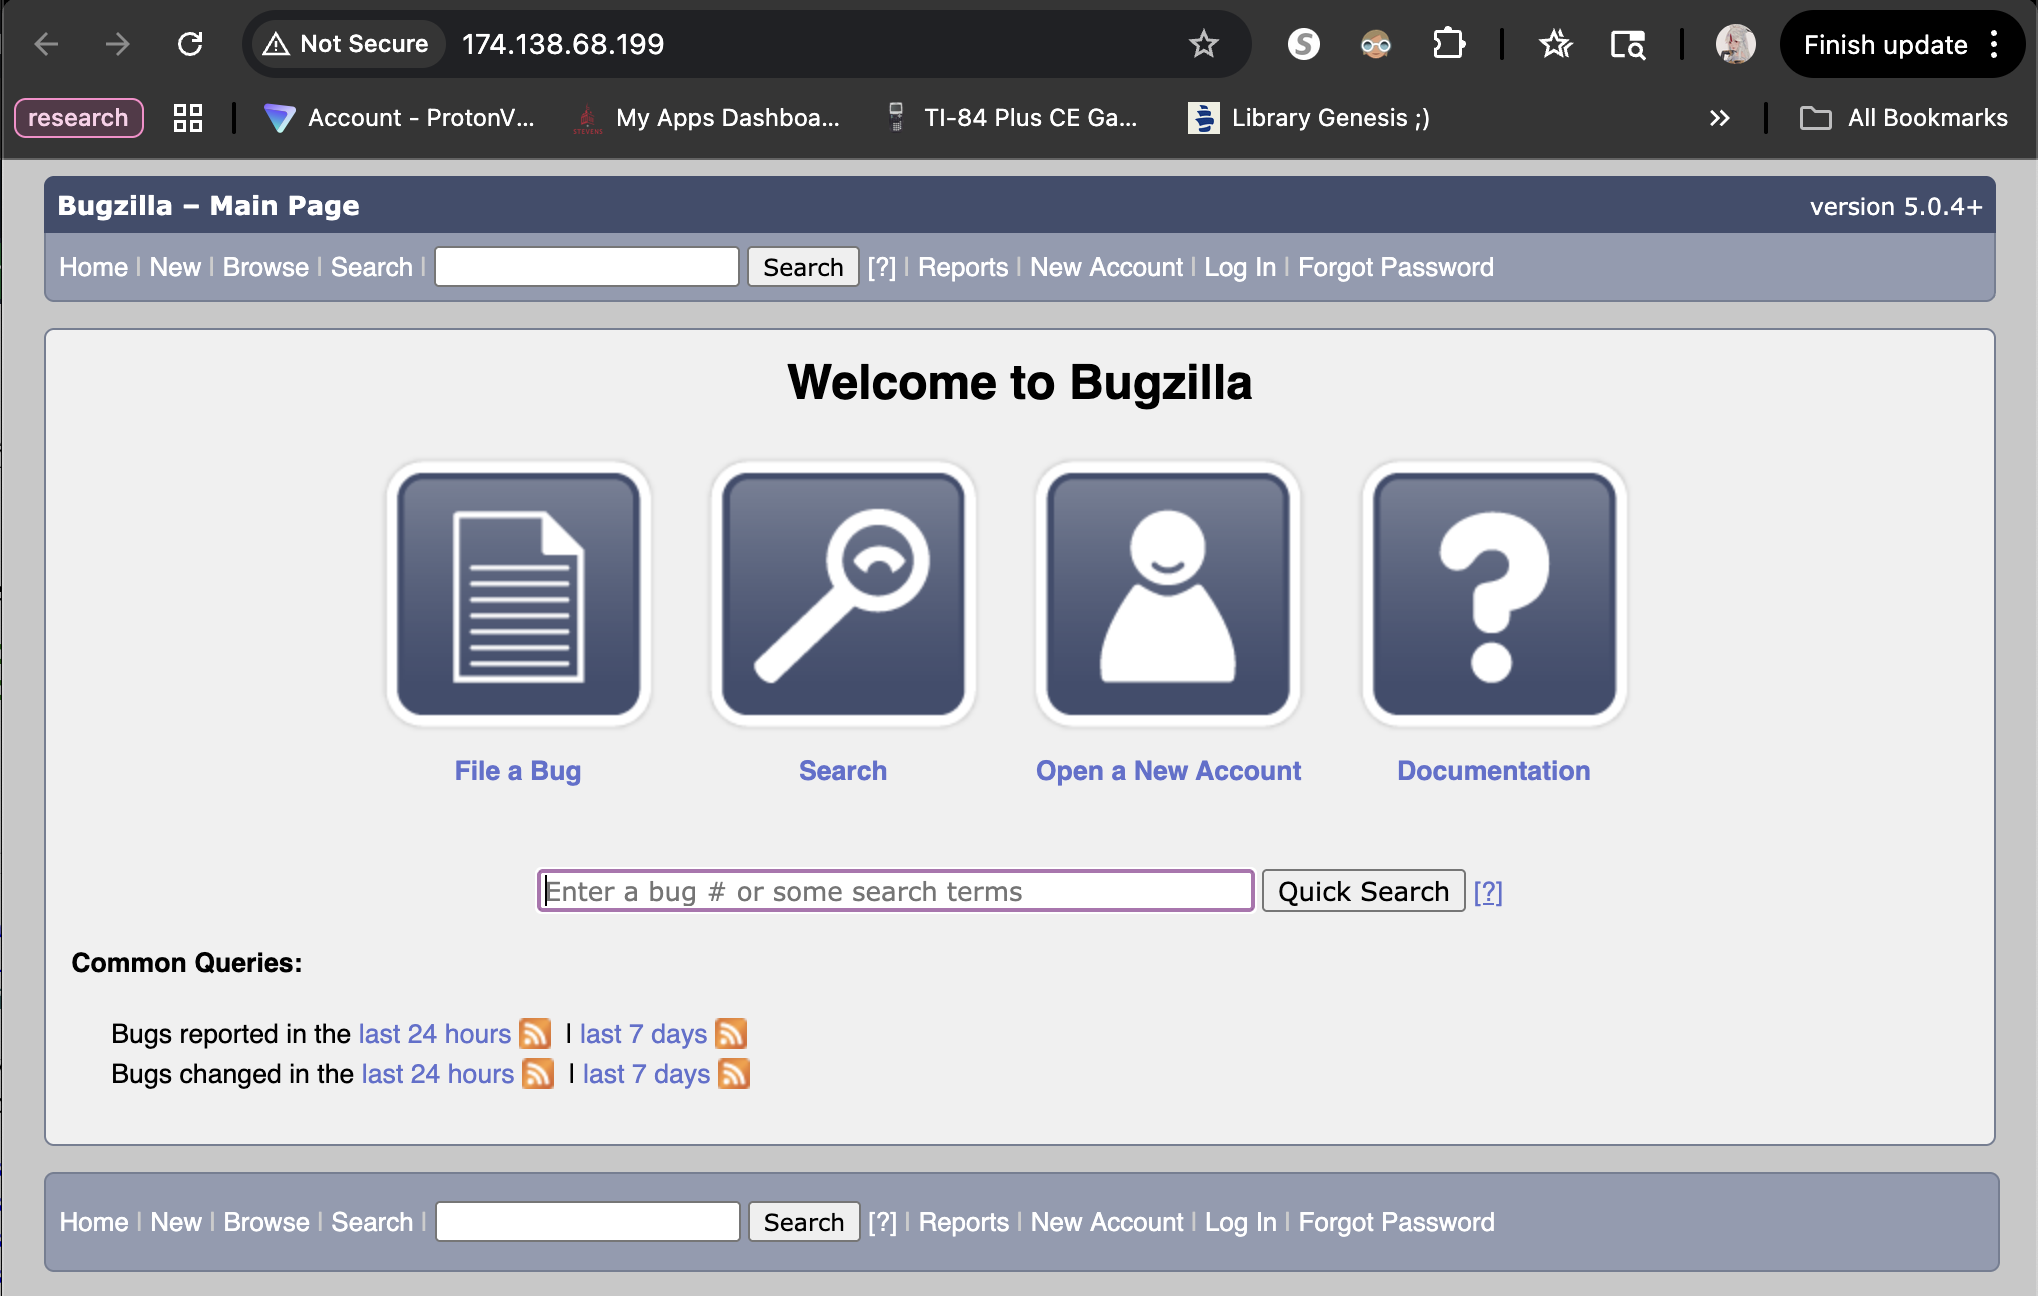
\includegraphics[width=0.7\linewidth]{png/bugzilla_landing.png}
    \caption{bugzilla website on http://174.138.68.199/}
    \label{fig:placeholder}
\end{figure}

\noindent logged in with the given email and password, then head to Administration → Users and re-setted the password and email to real ones.

\noindent and now everything is running on http://174.138.68.199/. :)




